% Chapter Template

\chapter{Testing Drift Diffusion Solver} % Main chapter title

\label{Chapter4} % Change X to a consecutive number; for referencing this chapter elsewhere, use \ref{ChapterX}

\lhead{Chapter 4. \emph{Testing Drift Diffusion Solver}} % Change X to a consecutive number; this is for the header on each page - perhaps a shortened title

In the past chapter went through the details of how to solve drift-diffusion and Poisson's equation using finite difference method. In this chapter steady state and transient analysis for drift diffusion equations using finite differnce is compared to analytical solutions as well as a commercially available simulator called 'COMSOL Multiphysics' which uses finite element method instead of finite difference. Following test cases were made to ensure that the key parts of the finite difference scheme runs properly and does not produce unexpected results. 

\section{Solution for Closed Boundary}
In this section the accuracy of the finite difference solution in steady state will be tested. In order to do this simple 1-D problem where with a finite number of negatively charged particles over a certain distance subject to constant electric field is used. This is the same problem that was solved analytically in section 3.3.1. It is also assumed that the charge density is very low and does not affect the electric field. Both ends of the simulation domain have no flow boundary conditions for charged particles. The solution process requires an initial distribution for charge density over the area. For this problem the density of the negative particles was initialized to be uniform over the entire area. 

Since the differential equations are uncoupled solving Poisson's equation only once is sufficient to determine the electric field over the course of the entire simulation. Figures \ref{5E} and \ref{5pot} show the potential and the electric field distribution over the entire simulation area calculated from Poisson's equation using finite difference. 

\begin{figure}
\centering
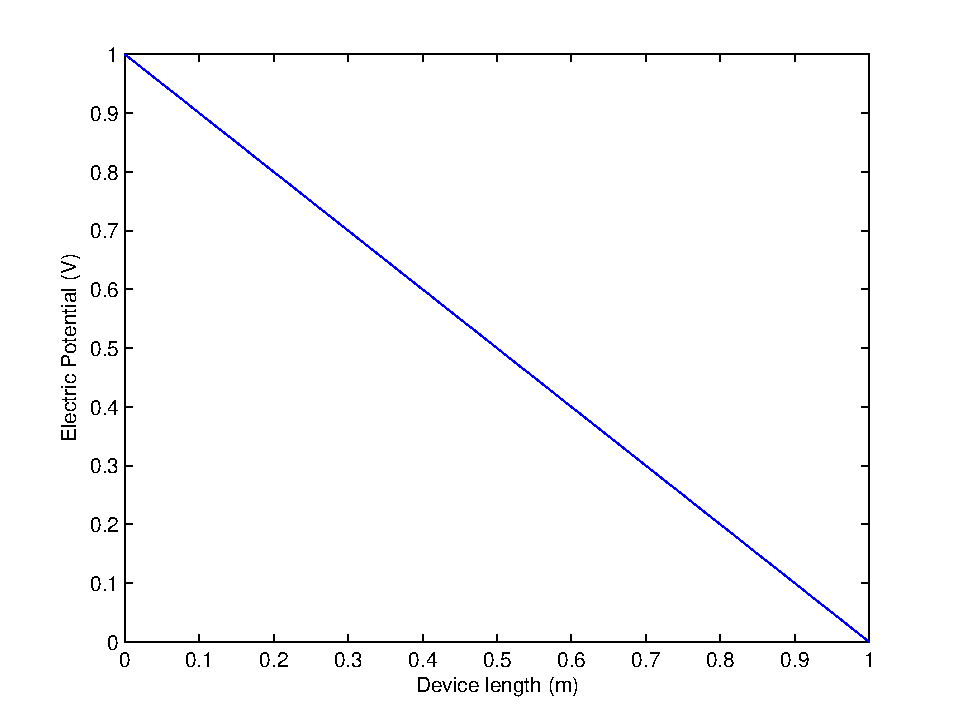
\includegraphics[scale=0.8]{5101}
\caption{Potential Distribution} 
\label{5pot}
\end{figure}

\begin{figure}
\centering
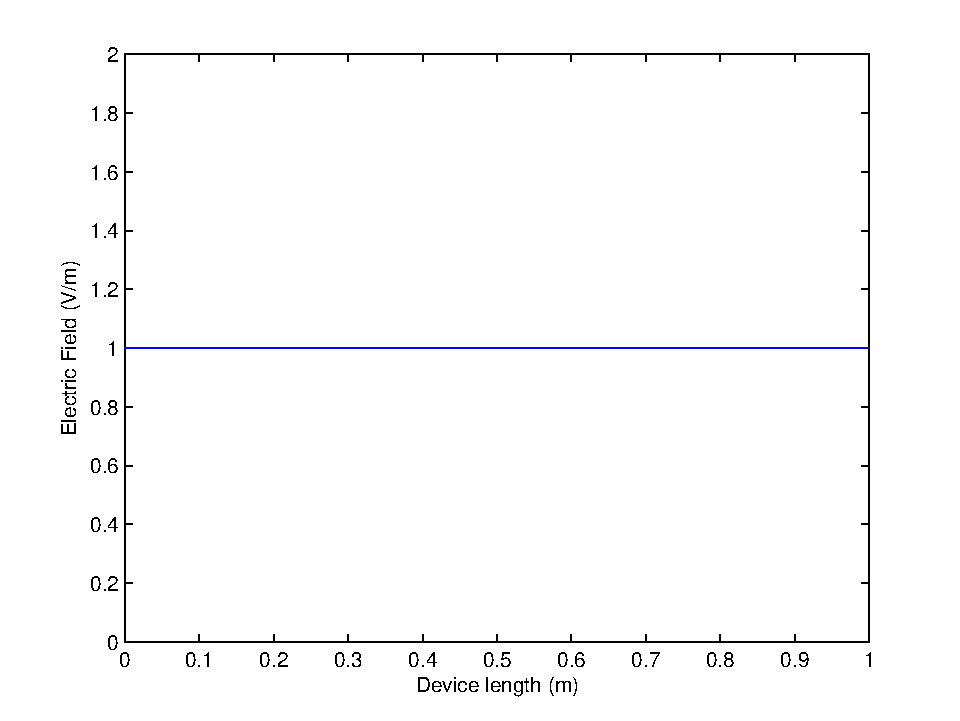
\includegraphics[scale=0.8]{5102}
\caption{Electric Field Distribution} 
\label{5E}
\end{figure}

\clearpage

Figure  \ref{5ss} has two simulation results as well as the exact solution of this problem. The green line represents the result given by the finite difference method at steady state. It can be seen from the graph that the steady state solution generated by both COMSOL and finite difference matched the analytical solution.

\begin{figure}
\centering
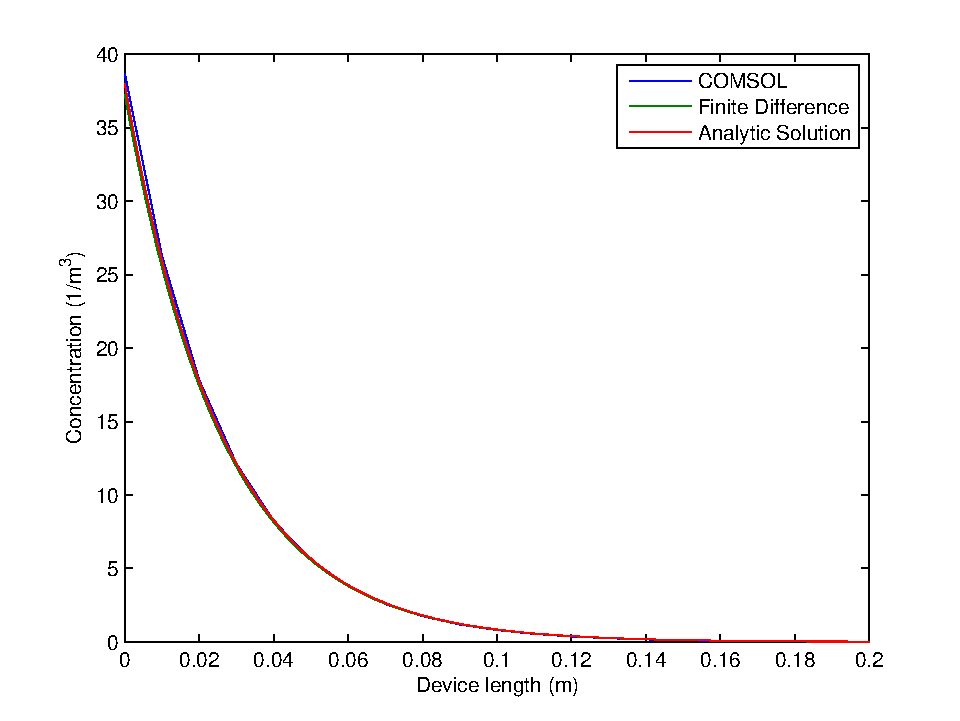
\includegraphics[scale=0.8]{511}
\caption{Steady State Negative Charge Density} 
\label{5ss}
\end{figure}

\begin{figure}[!htp]
\centering
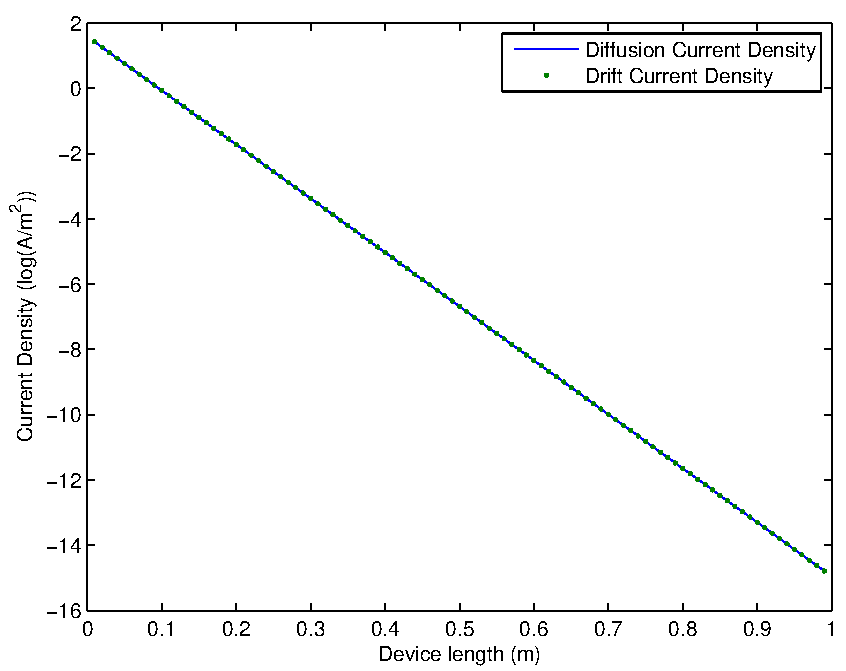
\includegraphics[scale=0.8]{513}
\caption{Finite Difference Drift and Diffusion Current Densities}
 \label{5curdens}
\end{figure}

While deriving an analytical solution for this problem we have assumed that at steady state the drift current density must be equal to the diffusion current density. In figure \ref{5curdens} we see drift and diffusion current densities in log scale. Overall both currents match quite tightly.

\textbf{(Add problems with high electric fields and debye length)}
\newline
\textbf{(This example tested the simulation for, steady state dn/dt=0 etc.. Generates good results for low E field but problems with high E fields)}

\clearpage
\section{Solutions for Open Boundary}
Another crucial aspect of drift-diffusion simulation is its transient response. Like the previous test case, the analytic solution can be used to test the accuracy of the transient response. Two different analytic solutions for a similar drift diffusion problems which involved infinite boundaries and a uniform electric field were generated in section 3.3.2. The only difference between two cases are their initial carrier distributions. One has a rectangular and the other one has a gaussian initial carrier distribution. Finite difference scheme does not allow simulation over an infinitely long conductor. For this simulation, a solution will be generated until the carrier distribution gets close to a wall.   

\begin{figure}[ht]
\centering
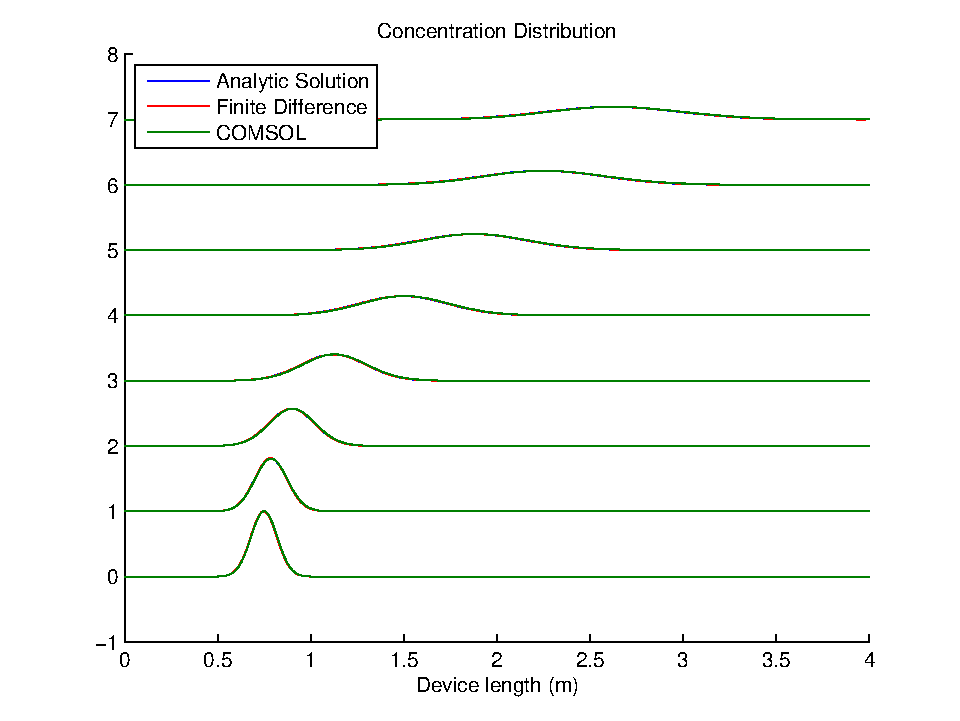
\includegraphics[scale=0.8]{5212}
\caption{Gaussian Carrier Distribution Evolving Over time} 
\label{51}
\end{figure}

Figure \ref{51} has the transient response from COMSOL, finite difference and analytical solution. Snapshots of the carrier distributions were taken for each method at different time steps and they were superposed on top of each other. Increasing levels on y axis represent a carrier distributions at a different time starting from the bottom and moving forward in time towards the top. Figure \ref{51} has a gaussian initial carrier distribution. It can be seen from that the transient solution generated by both COMSOL and finite difference are quite close to the analytical solution.

\textbf{(Needs conclusion, What this example showed ?)}

\clearpage
\section{PN Junction}
In previous test cases, Poisson's equation was not coupled with drift diffusion equations. In this example both drift diffusion and Poisson's equation will be tested to investigate how well they work when they are coupled together. A simple pn junction is quite adequate for this task since it has analytical solutions (under certain assumptions) for electric potential, electric field and carrier distribution.

For the simulation ,the initial hole and electron distributions were determined using mass action law and they were assumed to be constant at the boundaries. Keeping carrier concentrations constant at the boundaries creates a mechanism in which the charge can move in and out of the simulation domain. If the charge density at any time step is higher than the fixed density then the difference will move out of the system. If there is a lack of charge at the boundary then carriers will move in to fill in the gap. Following figure (\ref{npcon}) shows the final result of bringing p and n type materials together. 
 
\begin{figure}[ht]
\centering
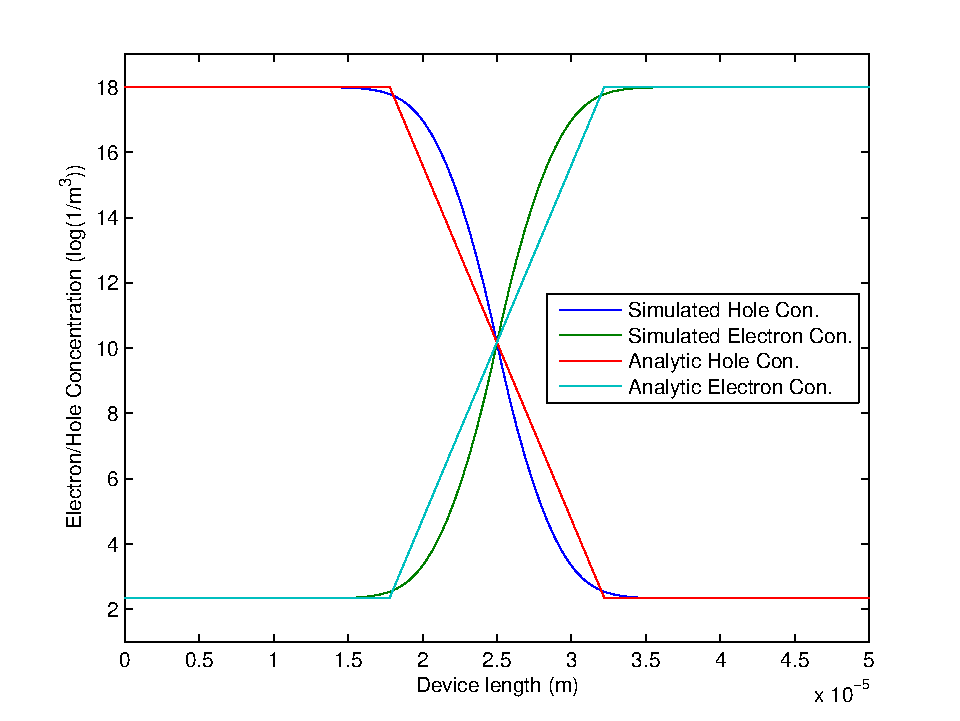
\includegraphics[scale=0.8]{5311}
\caption{Electron/hole Concentration of a PN Junction} 
\label{npcon}
\end{figure}

There is a little mismatch between simulated and analytic concentration densities. Analytic solution have sharp edges and simulated solution does not. This is due to all the assumptions made in order to find an analytic solution. This mismatch can also be seen for electric field, electric potential and net charge .

 Figure \ref{pnpot} shows the potential distribution for simulated and analytic solution. Close match in electric potential distribution shows that coupled equations can generate fairly accurate solutions.
 
\begin{figure}[!htp]
\centering
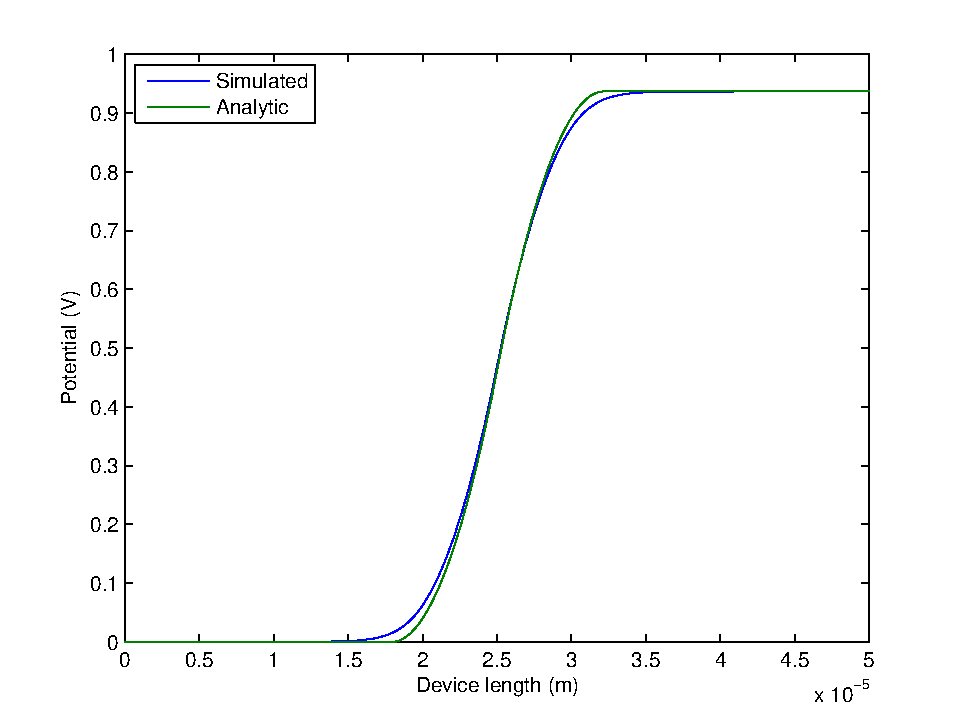
\includegraphics[scale=0.7]{5312}
\caption{Potential Distribution of a PN Junction} 
\label{pnpot}
\end{figure}

Calculation of the electric field involves one basic derivative. Since simulated potential is matching the analytic solution quite nicely the electric field should follow a similar pattern. Figure \ref{pnefield} shows that this is indeed the case, simulated electric field matches the calculated electric field.
\begin{figure}[!htp]
\centering
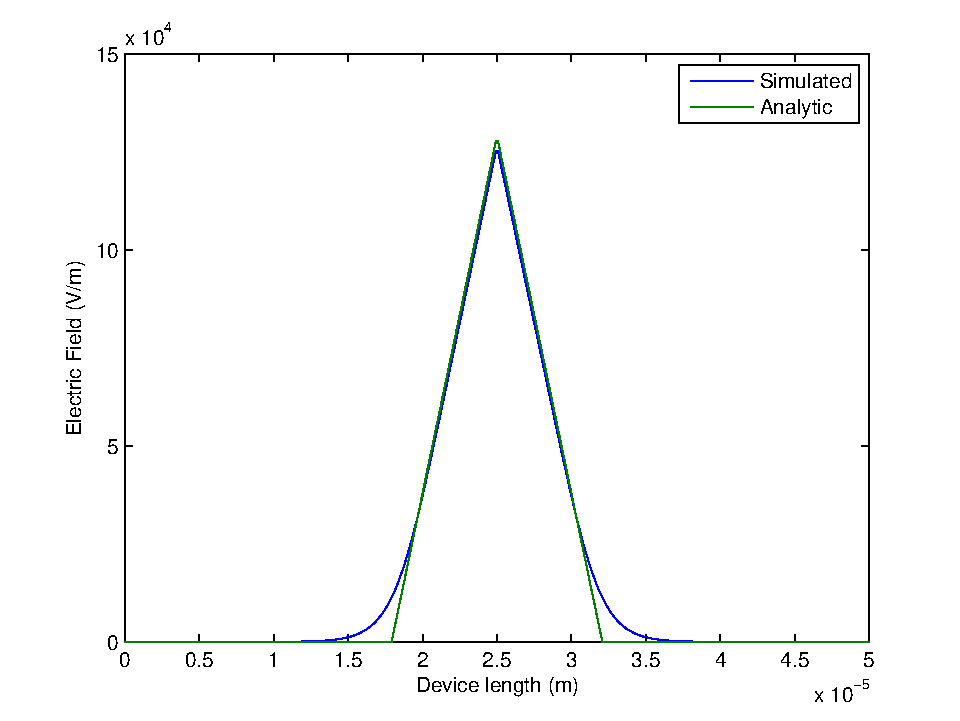
\includegraphics[scale=0.7]{5313}
\caption{Electric Field Distribution of a PN Junction} 
\label{pnefield}
\end{figure}

Figure \ref{pncd} shows the total charge distribution at steady state. Simulated net charge density follows the analytic one except the abrupt changes at two ends. 
\begin{figure}
\centering
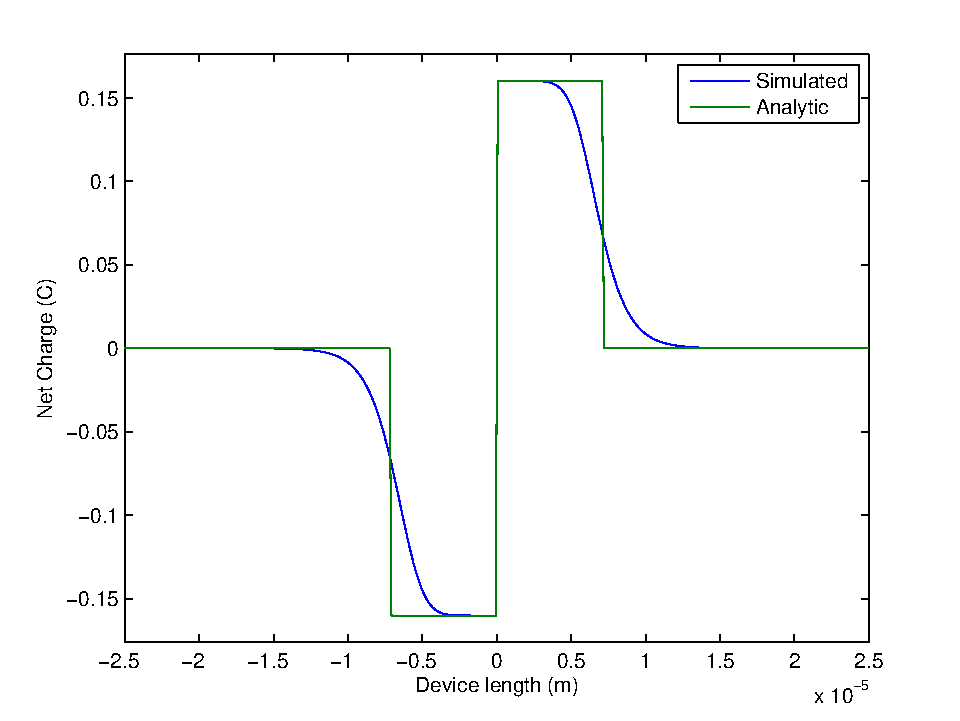
\includegraphics[scale=0.8]{5314}
\caption{Total Charge Distribution of a PN Junction} 
\label{pncd}
\end{figure}

\textbf{(Needs conclusion, What this example showed ?)}


\clearpage
\section{Region Specific Particle Density Limit}

The last property of the drift diffusion simulation scheme to be tested concerns the movement of lithium ions. As lithium ions move into the PEDOT:PSS they bond with PSS polymers and replace holes. PEDOT:PSS can only absorb lithium as long as there are available PSS polymers to bond with therefore PEDOT:PSS has limited capacity to accept lithium ions. This behavior can be captured during simulation by using a Dirichlet boundary condition (J=0) to stop the particle flow into a node if the density will go over a preset limit. This can be achieved in two different ways. 

A soft limit can be set by making particle mobility a function of its density. This function can be defined such a way that it switches from high to a low value when the particle density approaches its limit. This implementation is straightforward and can be used in commercial simulators but it has a drawback. Once the particle density is reached the mobility and diffusivity of the lithium particles are stuck at very low values. If there is an outflux of particles from that particular node then the density is stuck at the limit until the mobility function goes back to a value which allows particle flow. This can introduces a considerable lag in the response of lithium current density.  

An alternative approach is precalculating the particle density of a density limited node at the next time step, setting any influx to zero if the density is going to go over the limit and finally recalculating the particle densities at the next time step using the updated current densities. This mechanism sets a hard limit on the density since there is a sudden cut instead of a gradual cut in the current flow. This density limiting mechanism is more responsive than the previous one but it requires the calculation of the next time step twice for the species that has a limit. Also large currents caused by either a big time step or high electric field can force the algorithm to cut the current flow into a node before the density reaches its limit.

To avoid adding any lag into the system latter method was chosen for memristor simulations in this thesis. This method was implemented in finite difference drift diffusion solver and it is tested in this chapter. Also a soft limit was implementend in COMSOL for comparison since it did not support the hard limit method.  

In order to test density limiting method implemented for memristor simulation a simple example was set up. Two positively charged particles were initialized like the figure below (\ref{5412}). One set of particles has a concentration limit of $2 \; 10^{10} \; m^{-3}$ on the right side of the simulation area and no limit on the left side. The other set has no restrictions.
\begin{figure}[!htp]
\centering
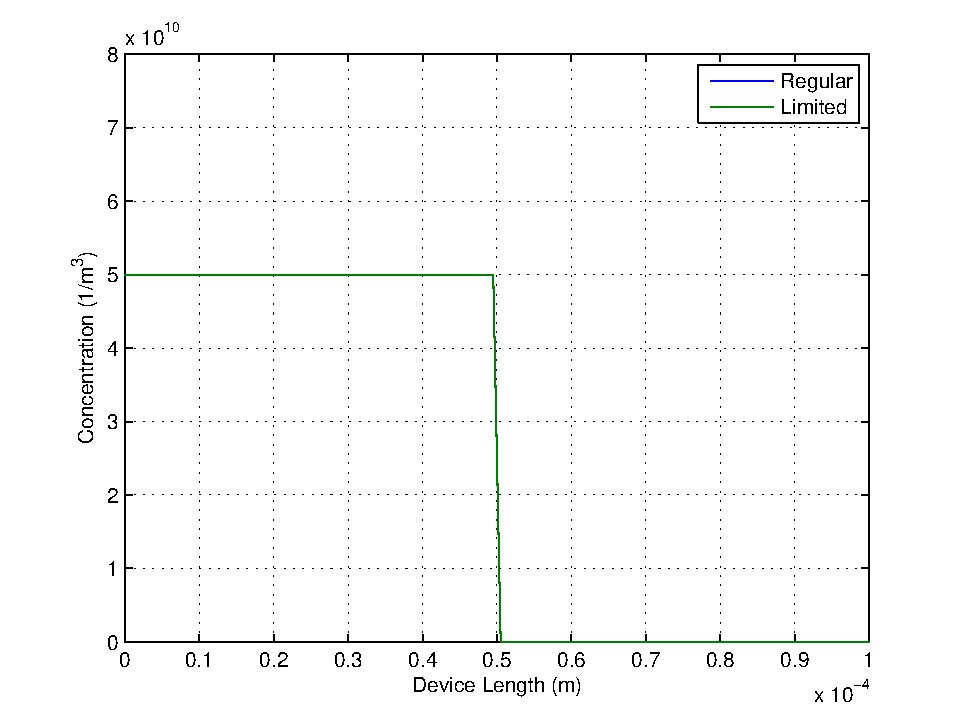
\includegraphics[scale=0.7]{5412}
\caption{Initial Particle Density} 
\label{5412}
\end{figure}

This transient simulation was done using a potential train. The potential is applied to the left side of the device and the right side is always grounded. For the first half of the simulation applied potential was positive and for the second half it was negative. Figure \ref{5412} shows how two simulations differ when the particles are pushed towards the right wall due to the electric field created by the positive potential. Particles with no limit on the right side move freely and accumulate on the right side. The limit for the other particles is effectively stopping them from going in and accumulating freely. Once the limit is reached at a certain node the density cannot increase any further and that node turns into a no flow wall. 

\begin{figure}[!htp]
\centering
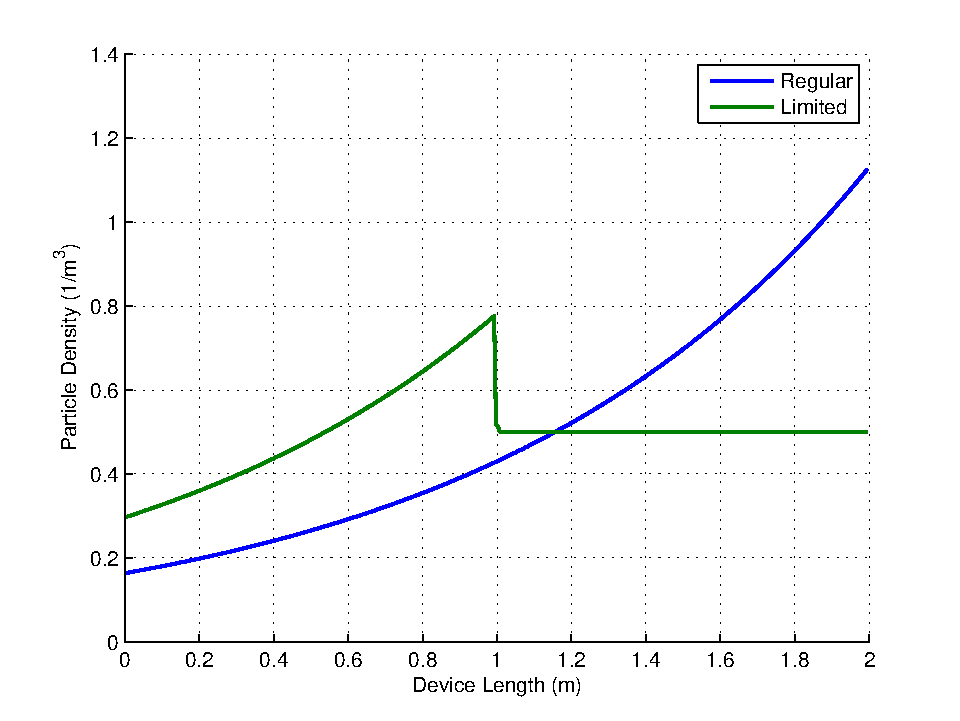
\includegraphics[scale=0.7]{5413}
\caption{Limited Concentration Accumulation on the Right Side} 
\label{5413}
\end{figure}

When the potential is switched all the particles accumulate freely to the left side of the simulation domain since there are no restrictions on this side (figure \ref{5414}).
\begin{figure}[!htp]
\centering
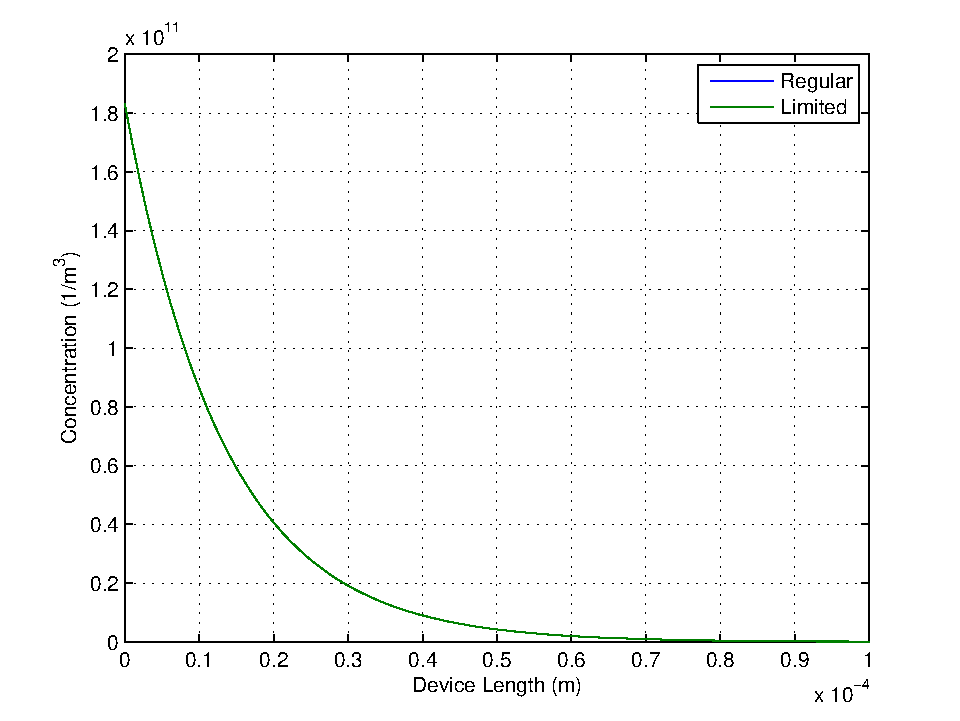
\includegraphics[scale=0.7]{5414}
\caption{Limited Concentration Accumulation on the Left Side} 
\label{5414}
\end{figure}

This last figure (\ref{5411}) shows the transient response  over time of a single node on the right side. The potential is positive for the first 1.5 seconds and it is switched to negative for the last 1.5 seconds. The node without limit keeps accepting charge until steady state has been reached but the node with a limit on stops accepting charged particles once the limit is reached. After the potential is switched density limited node has no problem releasing the particles.


\begin{figure}[!htp]
\centering
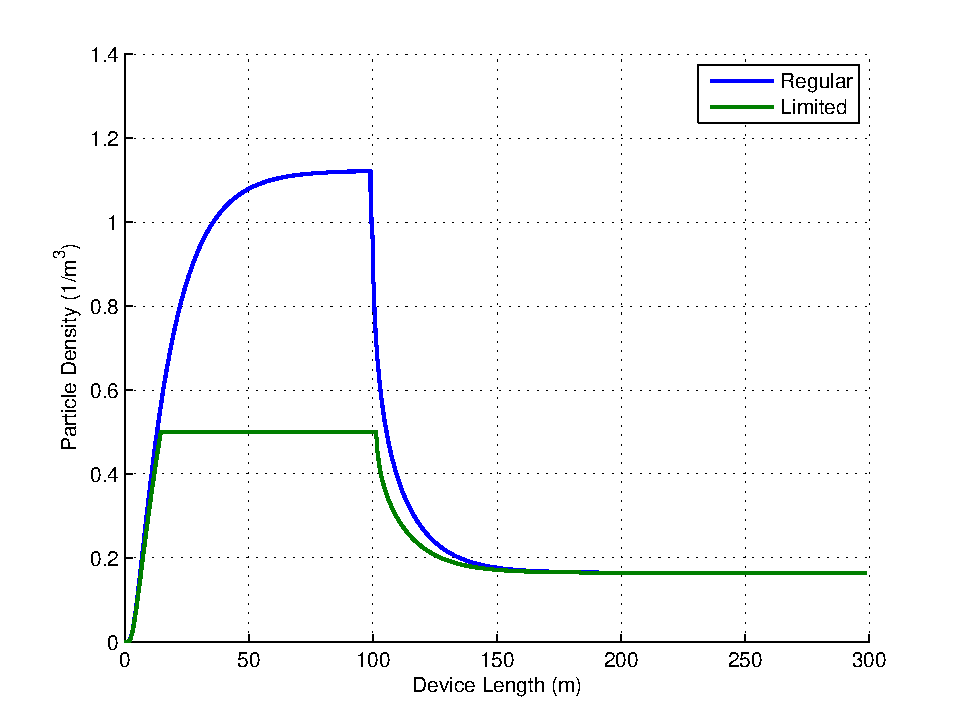
\includegraphics[scale=0.7]{5411}
\caption{Accumulation at the right wall over time} 
\label{5411}
\end{figure}

Additional to the test that was run for finite difference, COMSOL was used to test the soft limiting mechanism. COMSOL does not have a built in option that allows limiting particle density. One possible solution to this is making particle mobility and diffusivity a function particle density. It is possible to use a sigmoid function which switches from 1 to 0 very quickly when particle density is close to its limit. Here is the equation of the sigmoid function used to limit the particle flow:

\begin{equation}
\mu = \frac{\mu_{0}}{1+e^{\sigma(n-n')}}
\label{mur}
\end{equation} 

$\mu_0$ is the original mobility of the charge carrier. $\sigma$ controls the sharpness of the switch and $n'$ determines the density at which the switch will be. 

Another problem with COMSOL was the definition of mobility and diffusion coefficients over different areas. If these constants are defined as one single value per area COMSOL simulates without any errors but if they are defined as a function of concentration it causes convergence issues. This can be overcome by using two more sigmoid functions to distinguish between two areas with different mobilities and diffusion constants. Left sigmoid in figure \ref{5420}  was multiplied by the mobility/diffusivity of the left side of the area and the right sigmoid was multiplied by the mobility/diffusivity of the right side of the area. Both functions were summed to obtain a function which describes the characteristics of the entire area.

\begin{equation}
\mu=\frac{\mu_{l}}{1+e^{\sigma_x(x-x')}}+\frac{\mu_{r}}{1+e^{-\sigma_x(x-x')}}
\end{equation}

In this problem $\mu_r$ is the same as equation \ref{mur} since the region on the right side has a particle density limit. A sharp switch between right and left side mobility using the function above would be ideal for this simulation but unfortunately it causes convergence issues in COMSOL therefore there is a gradual change between two mobilities. 

\begin{figure}[!htp]
\centering
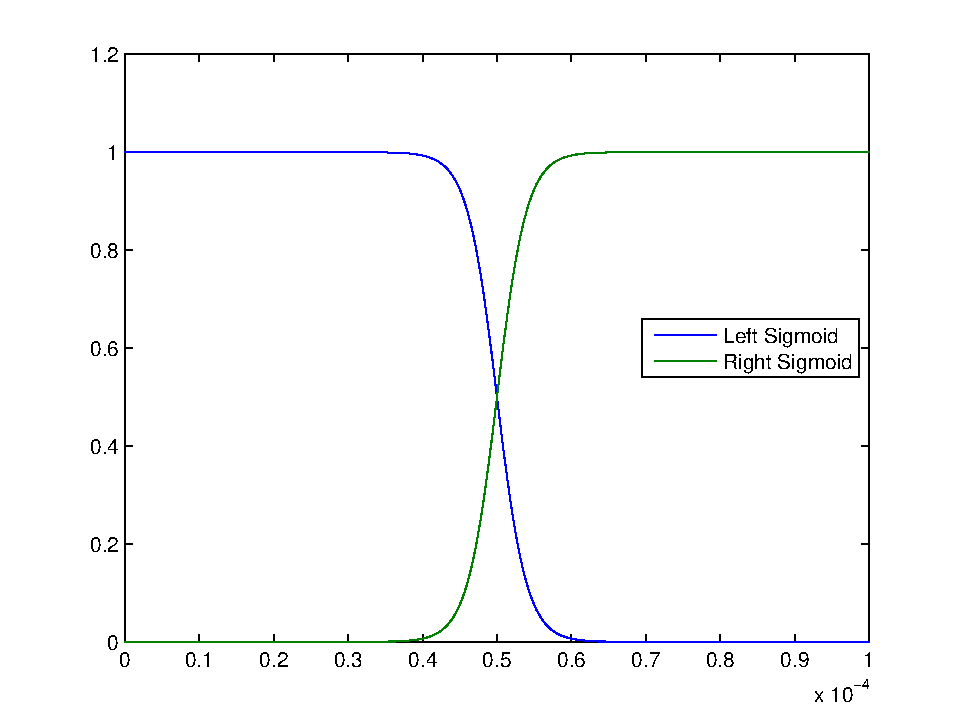
\includegraphics[scale=0.7]{5420}
\caption{Mobility change from left to right side} 
\label{5420}
\end{figure}

The initial carrier distribution for COMSOL was set to be exactly the same as finite difference simulation. Figures \ref{5416} and \ref{5423} show results for both COMSOL and finite difference simulations at steady state before the potential switch. The plot on the left side gives insight on how COMSOL simulation behaves for limited and limitless accumulation on the right wall. Due to the gradual change of mobility and diffusion constants between two areas we end up with concentration on the right side higher than the limit which is $2 \; 10^{10}$. Additionally, the particle density goes over its limit near the right wall. In figure \ref{5423} the difference between COMSOL and finite difference becomes more visible. In FD simulation the accumulation goes much higher due to higher electric field and unlike COMSOL it does not penetrate the right half of the simulation domain. 

\begin{figure}[ht]
\centering
\begin{minipage}[b]{0.45\linewidth}
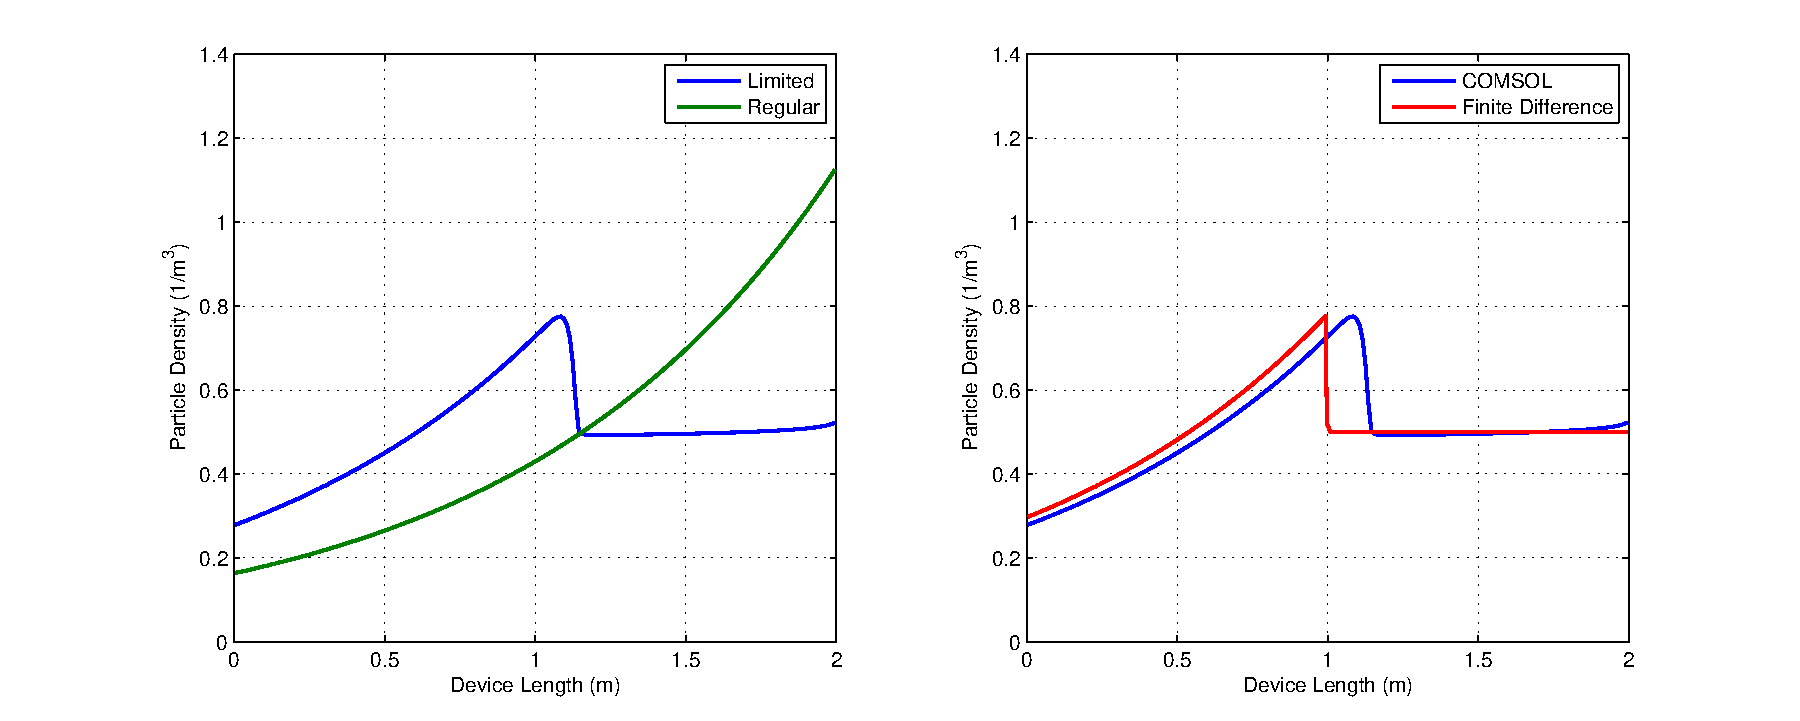
\includegraphics[scale=0.45]{5416}
\caption{COMSOL Simulation for Particle Density Limit}
\label{5416}
\end{minipage}
\quad
\begin{minipage}[b]{0.45\linewidth}
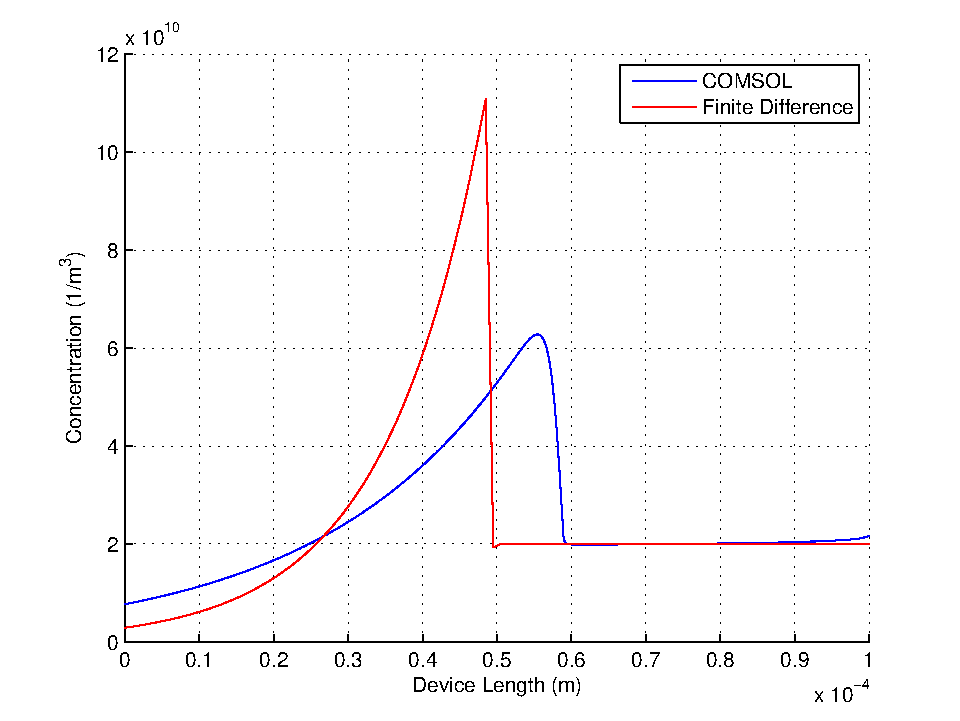
\includegraphics[scale=0.45]{5423}
\caption{COMSOL and Finite Difference Simulation}
\label{5423}
\end{minipage}
\end{figure}


In figure \ref{5417} it is possible to see the accumulation of charge near the middle after the potential is switched. This is due to mobility being a function of distance and concentration. As the ions move from left to right they go from a low mobility region to a high mobility region and they slowly accumulate around the area where the change in mobility occurs. Figure comparing both COMSOL and finite difference shows that the accumulation does not happen in the case of finite difference due to the way concentration limiting mechanism was implemented.

\begin{figure}[ht]
\centering
\begin{minipage}[b]{0.45\linewidth}
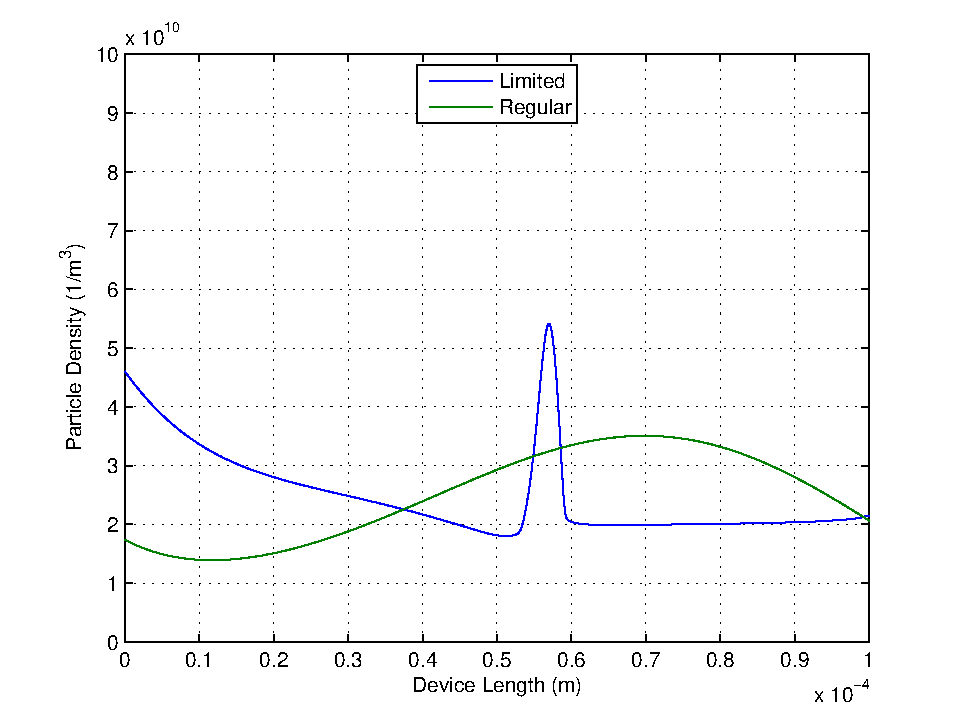
\includegraphics[scale=0.45]{5417}
\caption{COMSOL Simulation for Particle Density Limit}
\label{5417}
\end{minipage}
\quad
\begin{minipage}[b]{0.45\linewidth}
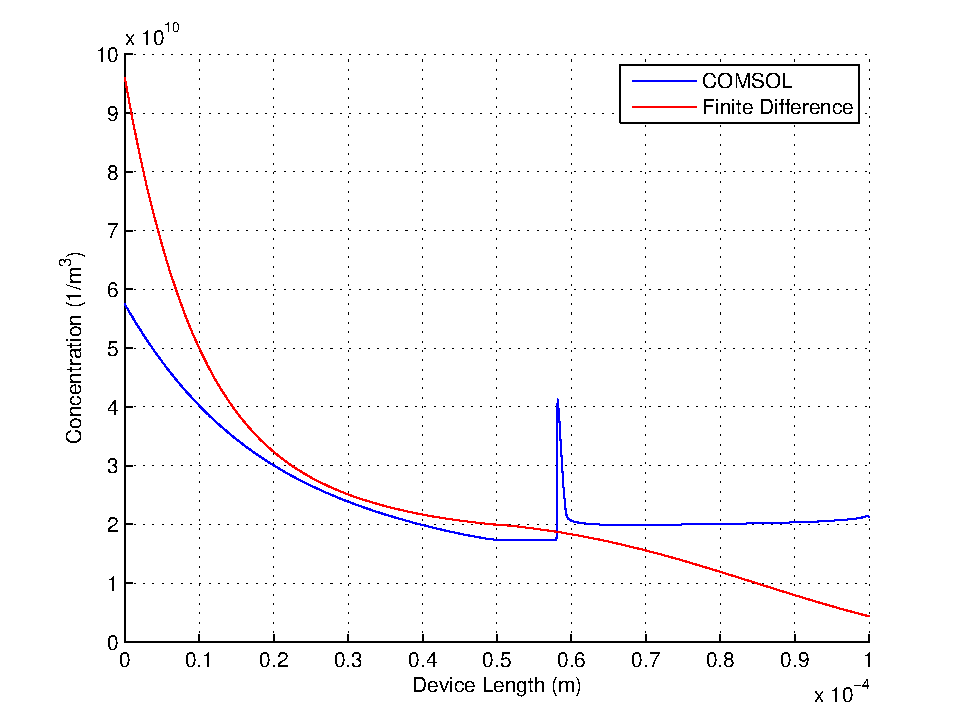
\includegraphics[scale=0.45]{5424}
\caption{COMSOL and Finite Difference Simulation}
\label{5424}
\end{minipage}
\end{figure}

With the decrease of ion concentration on the limited region the difference between low and high mobility regions diminish. Once the concentration on the limited side is low enough the whole system behaves as if there was no limit and ion mobility becomes equal for all regions and the ions freely accumulate on the left wall (figure \ref{5418}). Aside from the difference in electric field strength both simulations behave the same way as they approach steady state. Figure \ref{5426} shows concentration densities at steady state. COMSOL simulation has a lower electric field since it has convergence issues with high electric fields. 

\begin{figure}[ht]
\centering
\begin{minipage}[b]{0.45\linewidth}
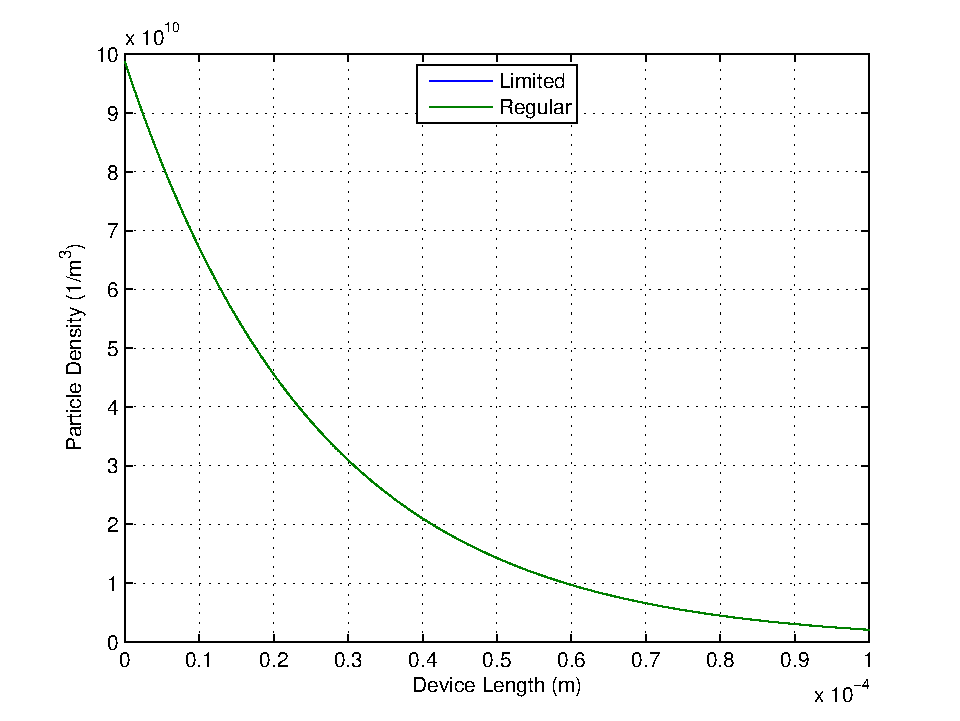
\includegraphics[scale=0.45]{5418}
\caption{COMSOL Simulation for Particle Density Limit}
\label{5418}
\end{minipage}
\quad
\begin{minipage}[b]{0.45\linewidth}
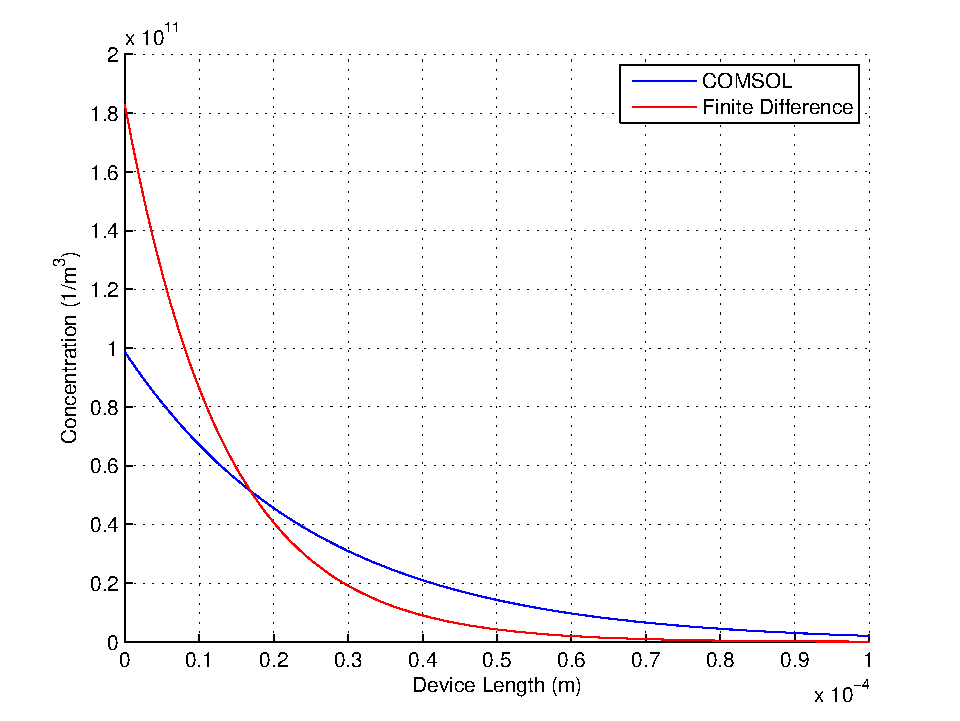
\includegraphics[scale=0.45]{5426}
\caption{COMSOL and Finite Difference Simulation}
\label{5426}
\end{minipage}
\end{figure}

This comparison can be finalized by looking the particle density transient response of the rightmost node. For the first half of the simulation everything is the same as the finite difference case except COMSOL goes a little bit over the limit. When the potential is switched, node without the limit has no noticeable difference in behaviour. The node with concentration limit has a lag when it comes to releasing the particles. This is due to the sigmoid function used to achieve a limiting behaviour. Once the limit is reached mobility and diffusivity are stuck at a very low value until the particle density starts to go lower than the limit.
\begin{figure}[ht]
\centering
\begin{minipage}[b]{0.45\linewidth}
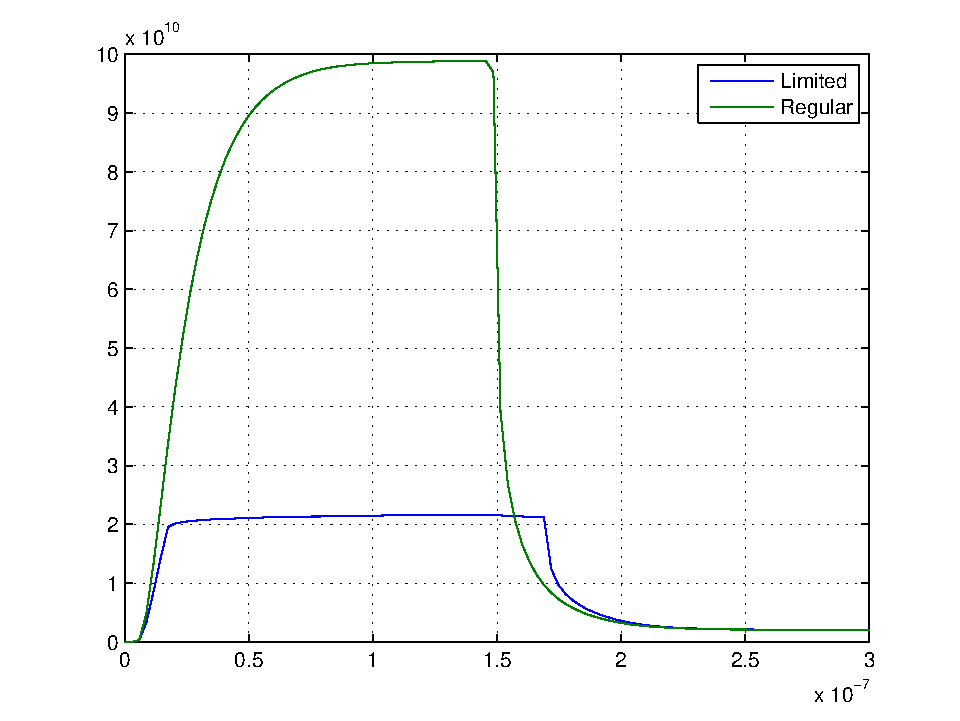
\includegraphics[scale=0.45]{5419}
\caption{Density on the right wall over time using COMSOL}
\label{5419}
\end{minipage}
\quad
\begin{minipage}[b]{0.45\linewidth}
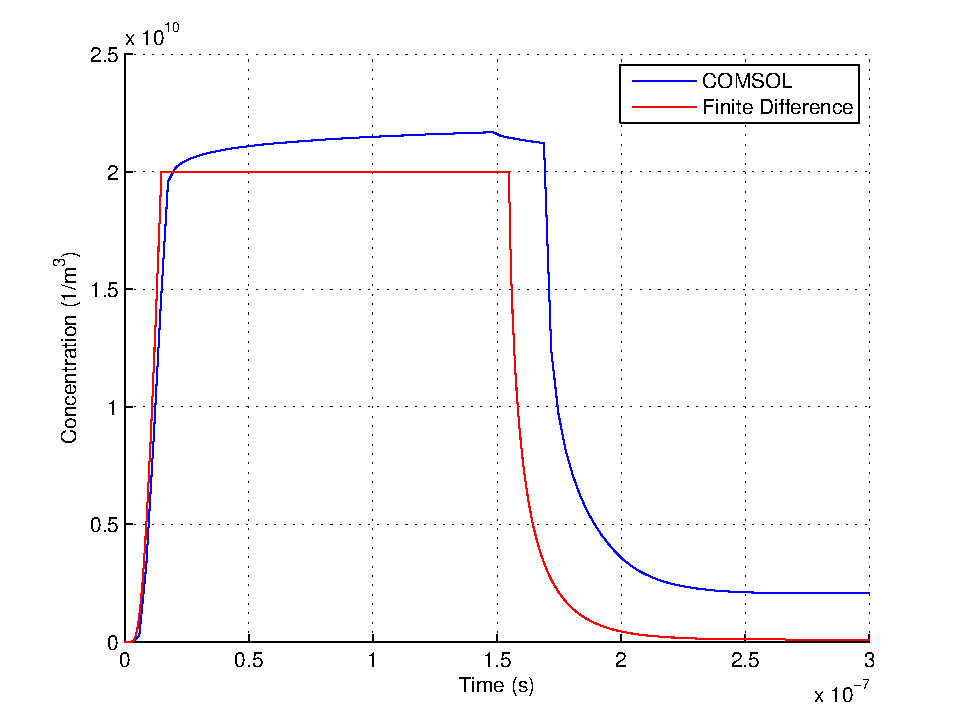
\includegraphics[scale=0.45]{5421}
\caption{Density on the right wall over time,COMSOL vs. Finite Difference}
\label{5421}
\end{minipage}
\end{figure}

The simulations above showed that is possible to impose a density limit over any area using a simple no flow boundary condition in finite difference. For COMSOL some workarounds had to be implemented in order to simulate the same behavior which caused convergence issues. 

\textbf{(Need a better conclusion)}